\section{Conclusions and Future Work}
\label{conclusions}


\begin{table*}[]
  \centering
  \begin{tabular}{|c|c|p{.6\textwidth}|}
    \hline
    Extension & Base Approach & Summary \\
    \hline
    \sparqlstr & \sparql1.1 & Window definitions with variable upper boundary\newline
    Window-to-stream operators\\
    \hline
    \stwoo & \rtwoo & Stream definitions in mapping \newline
    Streaming data types \newline
    Virtual \rdf stream \iri\!\!s\\
    \hline
    & \odemapster & Translation of \sparqlstr queries into \sneeql \\
    \hline
  \end{tabular}
  \caption{Summary of key contributions.}
  \label{tab:tabla}
\end{table*}


We have presented an approach for providing ontology-based access to streaming data, which is based on \sparqlstr, a
\sparql extension for \rdf streams, and \stwoo, an extension to \rtwoo for expressing mappings from streaming sources
to ontologies. We have shown the semantics of the proposed extensions and the mechanism to generate data source queries
from the original ontological queries using the mappings. The case presented here generated \sneeql queries but the
techniques are independent of the target stream query language, although issues of stream data model and language
evaluation semantics would need to be considered for each case. Finally the prototype implementation, which extends
\odemapster, has shown the feasibility of the approach. This work constitutes a first effort towards ontology-based
streaming data integration, relevant for supporting the increasing number of sensor network applications being
developed and deployed in the recent years. The extensions presented in this paper can be summarized in Table \ref{tab:tabla}.

This approach is being used in the context of two applications that are being developed in the SemSorGrid4Env\footnote{\url{http://www.semsorgrid4env.eu} accessed 29 September 2010.} (Semantic Sensor Grids for Rapid Application Development for Environmental Management) project. The first is the Flood Warning Use Case\cite{Hutton_10} which incorporates a network of heterogeneous sensors run by the Channel Coastal Observatory which are already in operation, and datasets collected by this project from data already in existence. These sensors are deployed in buoys at 36 locations of the South East England coast, measuring wave height, direction spread, temperature, etc. One of the aims of the Use Case is to utilize the CCO data, in order to produce real-time flood risk predictions for The Solent, Southern UK as well as possibly supporting longer term coastal planning through the development of scenarios. The outcomes of the project will also enable users to combine datasets from different sources, by creating mashups. We can see a screenshot of the application in Figure \ref{fig:floodap}.
The second application is the Fire Monitoring Use Case\cite{Guillen_10} which is focused on creating a  fire monitoring and warning system in a forest region near Cercedilla in Spain.
The system aims to prevent and detect fire combining two real-world real-time data sources: satellite data and measurements taken from a deployed Wireless Sensor Network in the area.  

\begin{figure*}[t]
  \centering
  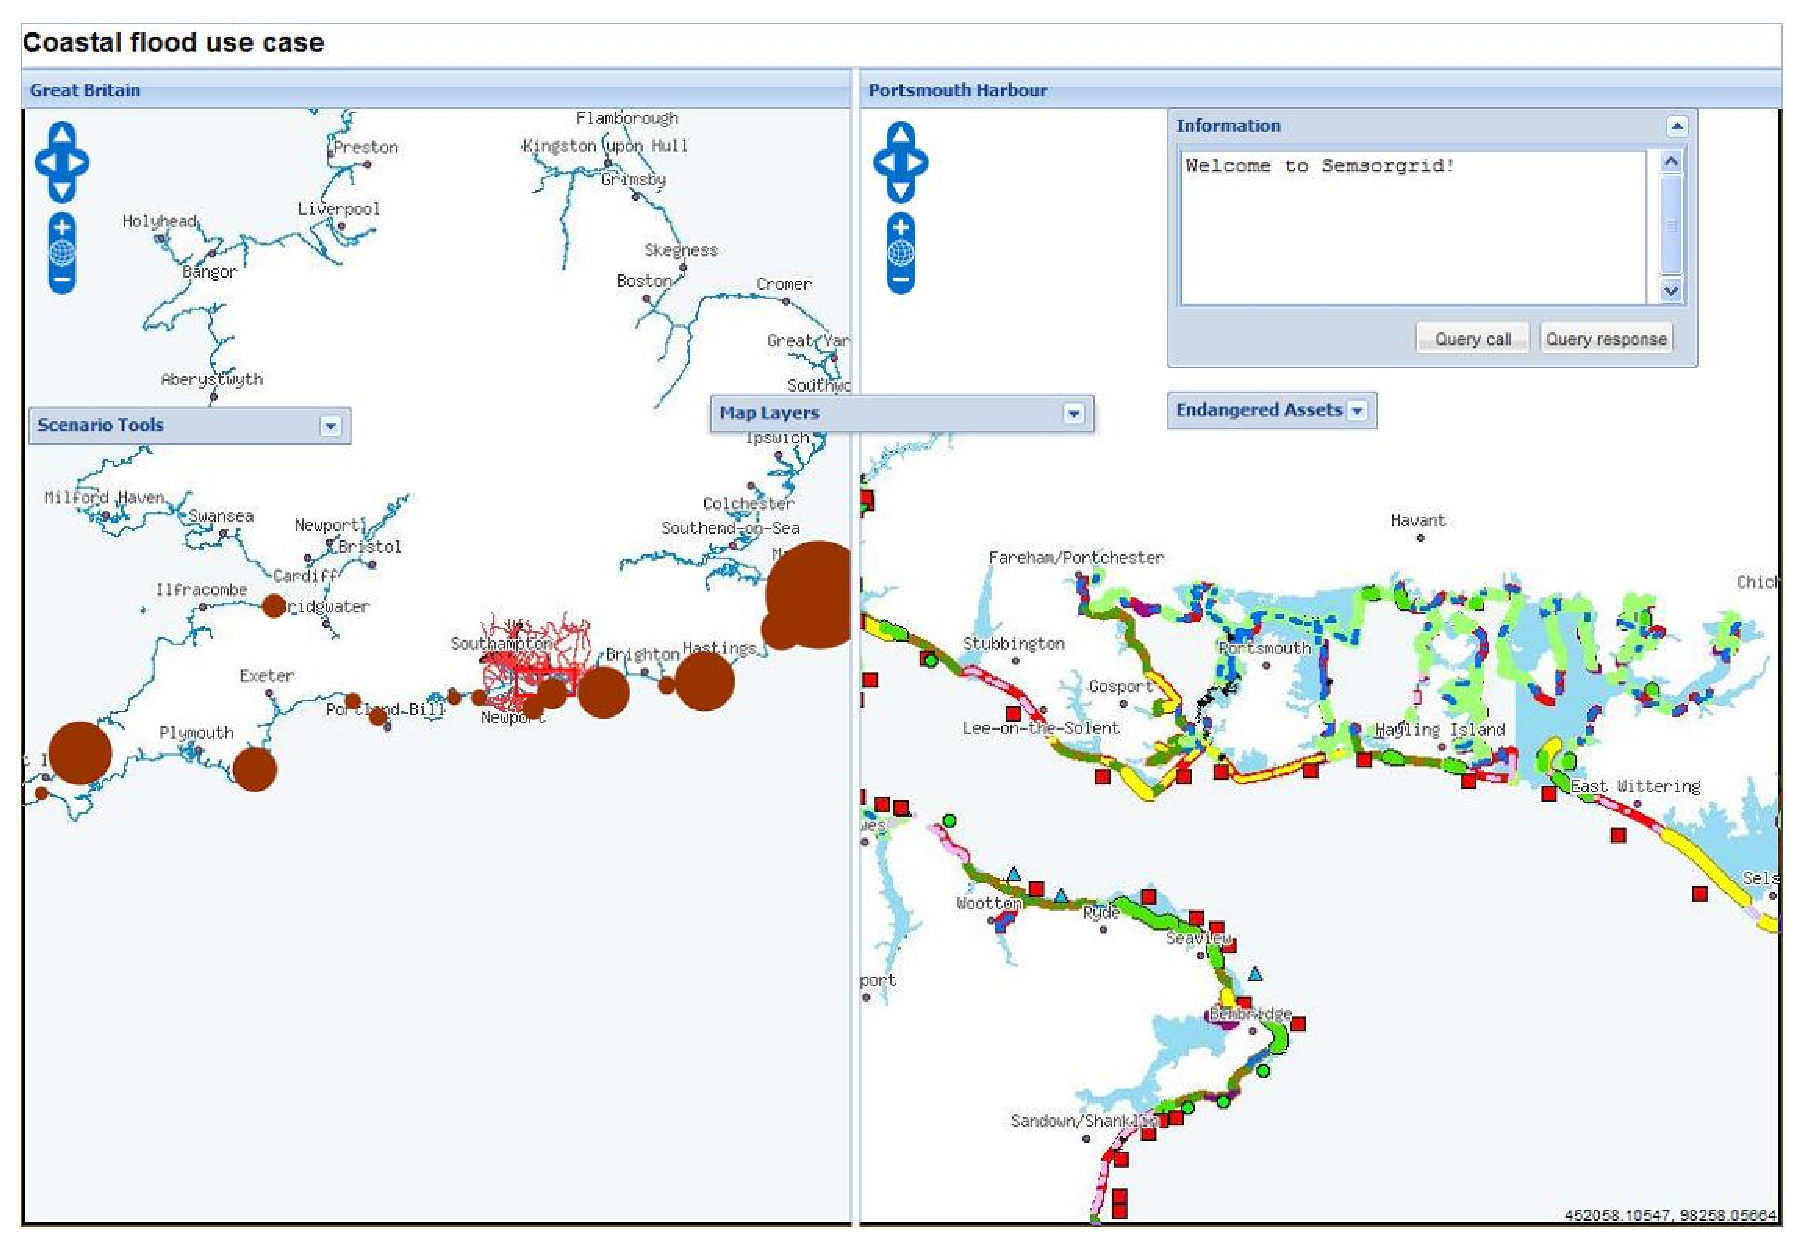
\includegraphics[width=0.8\textwidth]{img/floodapp}
  \caption{Flood Warning Use Case application. Red circles on the left map represent wave heights captured by the CCO sensors in the coast of South East England, queried and retrieved using the Ontology-based streaming data access service. On the right map, flood defences of the area are depicted.}
  \label{fig:floodap}
\end{figure*}

We are also preparing, with those data sources, a benchmark that will allow us to evaluate our approach in both query language expressiveness and performance. We will use the Linear Road Benchmark\cite{Arasu2004} as a basis but we will need extensions because it does not fit our evaluation focus. As our system delegates the query execution to the underlying stream engine, the focus of the evaluation is on the query and data translation.  

%\section{Future Work}
%\label{future}
%\bigskip
Although we have shown initial results querying the underlying \snee engine with basic queries, we expect to consider in the near future joins involving both streaming and stored data sources.
%We also plan to adapt our query rewriting approach to more recent and promising works such as \cite{PerezUrbina_09}.
Another important strand of future work is the optimization of distributed query processing \cite{Kossmann_00} and the streaming queries \cite{Abadi_2005,Galpin_09}.
It is also our goal to provide a characterization of our algorithms. 
In the scope of a larger streaming and sensor networks integration framework, we intend to achieve the following goals: %
i)~integrating streaming and stored data sources through an ontological unified view; %
ii)~combining data from event-based and acquisition-based streams, and stored data sources; %
iii)~considering quality-of-service requirements for query optimization and source selection during the integration.
%\fixme{This seems like a long future work list :/}
%The present work can be considered as a first step to our goal of providing an ontology-based integration platform for continuous heterogeneous data sources. 
%Therefore we will address the problems of heterogeneity, distributed query processing, and integration as part of this research track.

%%% Local Variables: 
%%% mode: latex
%%% TeX-master: "rere"
%%% End: 



%\vspace{-30pt}
